\documentclass{article}

% if you need to pass options to natbib, use, e.g.:
%     \PassOptionsToPackage{numbers, compress}{natbib}
% before loading neurips_2026

% The authors should use one of these tracks.
% Before accepting by the NeurIPS conference, select one of the options below.
% 0. "default" for submission
\usepackage{neurips_2026}
% the "default" option is equal to the "main" option, which is used for the Main Track with double-blind reviewing.
% 1. "main" option is used for the Main Track
%  \usepackage[main]{neurips_2026}
% 2. "position" option is used for the Position Paper Track
%  \usepackage[position]{neurips_2026}
% 3. "eandd" option is used for the Evaluations & Datasets Track
 % \usepackage[eandd]{neurips_2026}
% 4. "creativeai" option is used for the Creative AI Track
%  \usepackage[creativeai]{neurips_2026}
% 5. "sglblindworkshop" option is used for the Workshop with single-blind reviewing
 % \usepackage[sglblindworkshop]{neurips_2026}
% 6. "dblblindworkshop" option is used for the Workshop with double-blind reviewing
%  \usepackage[dblblindworkshop]{neurips_2026}

% After being accepted, the authors should add "final" behind the track to compile a camera-ready version.
% 1. Main Track
 % \usepackage[main, final]{neurips_2026}
% 2. Position Paper Track
%  \usepackage[position, final]{neurips_2026}
% 3. Evaluations & Datasets Track
 % \usepackage[eandd, final]{neurips_2026}
% 4. Creative AI Track
%  \usepackage[creativeai, final]{neurips_2026}
% 5. Workshop with single-blind reviewing
%  \usepackage[sglblindworkshop, final]{neurips_2026}
% 6. Workshop with double-blind reviewing
%  \usepackage[dblblindworkshop, final]{neurips_2026}
% Note. For the workshop paper template, both \title{} and \workshoptitle{} are required, with the former indicating the paper title shown in the title and the latter indicating the workshop title displayed in the footnote.
% For workshops (5., 6.), the authors should add the name of the workshop, "\workshoptitle" command is used to set the workshop title.
% \workshoptitle{WORKSHOP TITLE}

% "preprint" option is used for arXiv or other preprint submissions
 % \usepackage[preprint]{neurips_2026}

% to avoid loading the natbib package, add option nonatbib:
%    \usepackage[nonatbib]{neurips_2026}

\usepackage[utf8]{inputenc} % allow utf-8 input
\usepackage[T1]{fontenc}    % use 8-bit T1 fonts
\usepackage{hyperref}       % hyperlinks
\usepackage{url}            % simple URL typesetting
\usepackage{booktabs}       % professional-quality tables
\usepackage{amsfonts}       % blackboard math symbols
\usepackage{nicefrac}       % compact symbols for 1/2, etc.
\usepackage{microtype}      % microtypography
\usepackage{xcolor}         % colors
\usepackage{pifont}

\linenumbers
\newcommand{\cmark}{\textcolor{green}{\ding{51}}} % 勾选符号
\newcommand{\xmark}{\textcolor{red}{\ding{55}}}   % 叉号
\newcommand{\greencheck}{\textcolor{green}{\checkmark}}
\newcommand{\crosscheck}{\textcolor{red}{\XSolid}}

\newcommand{\tabincell}[2]{\begin{tabular}{@{}#1@{}}#2\end{tabular}}
\newcommand{\blank}[1]{\hspace*{#1}\linebreak[0]}

\newcommand{\pkd}[1]{\texttt{{\{\{\MakeUppercase{#1}\}\}}}}

\usepackage{adjustbox}
\usepackage{multicol}
\usepackage{multirow}%
\usepackage{array}
\usepackage{minted}
\usepackage[most]{tcolorbox}
\usepackage{listings}
\definecolor{softblue}{RGB}{100, 149, 237}
\definecolor{darkpurple}{RGB}{160, 0, 160}
\definecolor{darkred}{RGB}{160, 0, 0}
\definecolor{darkblue}{RGB}{0, 0, 160}
\definecolor{softgreen}{RGB}{120, 180, 100}
\usepackage{graphicx}
\usepackage{threeparttable}
\usepackage{amssymb} 
% \usepackage[colorlinks,linkcolor=black,anchorcolor=blue,citecolor=softblue]{hyperref}
% \tcbuselibrary{breakable}

\definecolor{darkgreen}{rgb}{0.0, 0.5, 0.0}
\definecolor{darkred}{rgb}{0.5, 0.0, 0.0}
% 定义颜色
\definecolor{bg}{rgb}{0.97,0.97,0.97}   % 背景色
\definecolor{codegray}{rgb}{0.3,0.3,0.3} % 代码灰色
\definecolor{codegreen}{rgb}{0,0.6,0}    % 代码绿色
\definecolor{backcolour}{rgb}{0.95,0.95,0.92} % 背景色

\def\xie{\textcolor{red}}
\def\xiao{\textcolor{orange}}
\def\deng{\textcolor{softgreen}}


% 定义 YAML 样式
\tcbuselibrary{listingsutf8}
\newtcolorbox{bg_yaml}{
  enhanced, % Enable advanced features
  sharp corners=southwest,
  colback=lightgray!20, % Background color
  colframe=black,       % Frame color
  boxrule=0.5mm,       % Frame thickness
  before=\vspace{1mm}, % Space before the box
  after=\vspace{1mm}   % Space after the box
}

% 定义 Python 样式
\lstdefinestyle{pythonstyle}{
    language=Python, 
    basicstyle=\ttfamily,  
    keywordstyle=\color{blue}, 
    commentstyle=\color{gray},   
    stringstyle=\color{red}, 
    showstringspaces=false,        
    numbers=left,                 
    numberstyle=\tiny\color{gray},
    stepnumber=1,                
    numbersep=5pt,               
    frame=single,                
    tabsize=4                     
}

\lstdefinestyle{yamlstyle}{
    basicstyle=\ttfamily\footnotesize,
    keywordstyle=\color{blue},
    commentstyle=\color{green!60!black},
    stringstyle=\color{red!60!black},
    numbers=left,
    numberstyle=\tiny\color{gray},
    breaklines=true,
}

\lstdefinelanguage{YAML}{
  keywords={true,false,null,y,n},
  keywordstyle=\color{blue}\bfseries,
  basicstyle=\ttfamily\small,
  commentstyle=\color{green!50!black},
  stringstyle=\color{red!60!black},
  identifierstyle=\color{black},
  numbers=left,
  numberstyle=\tiny\color{gray},
  breaklines=true,
  literate=
   *{:}{{{\color{blue}:}}}{1}
    {-}{{{\color{red}-}}}{1}
}


% Note. For the workshop paper template, both \title{} and \workshoptitle{} are required, with the former indicating the paper title shown in the title and the latter indicating the workshop title displayed in the footnote. 
\title{SelfAI: A self-directed framework for long-horizon scientific discovery}


% The \author macro works with any number of authors. There are two commands
% used to separate the names and addresses of multiple authors: \And and \AND.
%
% Using \And between authors leaves it to LaTeX to determine where to break the
% lines. Using \AND forces a line break at that point. So, if LaTeX puts 3 of 4
% authors names on the first line, and the last on the second line, try using
% \AND instead of \And before the third author name.


% \author{%
%   David S.~Hippocampus\thanks{Use footnote for providing further information
%     about author (webpage, alternative address)---\emph{not} for acknowledging
%     funding agencies.} \\
%   Department of Computer Science\\
%   Cranberry-Lemon University\\
%   Pittsburgh, PA 15213 \\
%   \texttt{hippo@cs.cranberry-lemon.edu} \\
%   % examples of more authors
%   % \And
%   % Coauthor \\
%   % Affiliation \\
%   % Address \\
%   % \texttt{email} \\
%   % \AND
%   % Coauthor \\
%   % Affiliation \\
%   % Address \\
%   % \texttt{email} \\
%   % \And
%   % Coauthor \\
%   % Affiliation \\
%   % Address \\
%   % \texttt{email} \\
%   % \And
%   % Coauthor \\
%   % Affiliation \\
%   % Address \\
%   % \texttt{email} \\
% }


\begin{document}


\maketitle

\begin{abstract}
    Scientific discovery increasingly entails long-horizon exploration of complex hypothesis spaces, yet most existing large language model (LLM) approaches emphasize final performance while offering limited insight into how scientific exploration unfolds over time, particularly balancing efficiency-diversity trade-offs and supporting reproducible, human-in-the-loop discovery workflows. We introduce SelfAI, a self-directed, multi-agent-enabled discovery system that automates scientific exploration as a strategic, trajectory-driven decision-making process. SelfAI translates high-level research intent into executable experiments, reasons over accumulated experimental trajectories to guide subsequent exploration, and applies adaptive stopping decisions to terminate unproductive search paths within a closed-loop workflow governed by explicit efficiency-diversity trade-offs. Evaluated using real-world experiments spanning domains from machine learning to drug discovery, SelfAI consistently discovers high-quality solutions with substantially fewer redundant trials than classical optimization methods and LLM baselines. Our work includes a project page and a VSCode extension~\url{}.
\end{abstract}

\section{Introduction}

\begin{figure*}
    \centering
    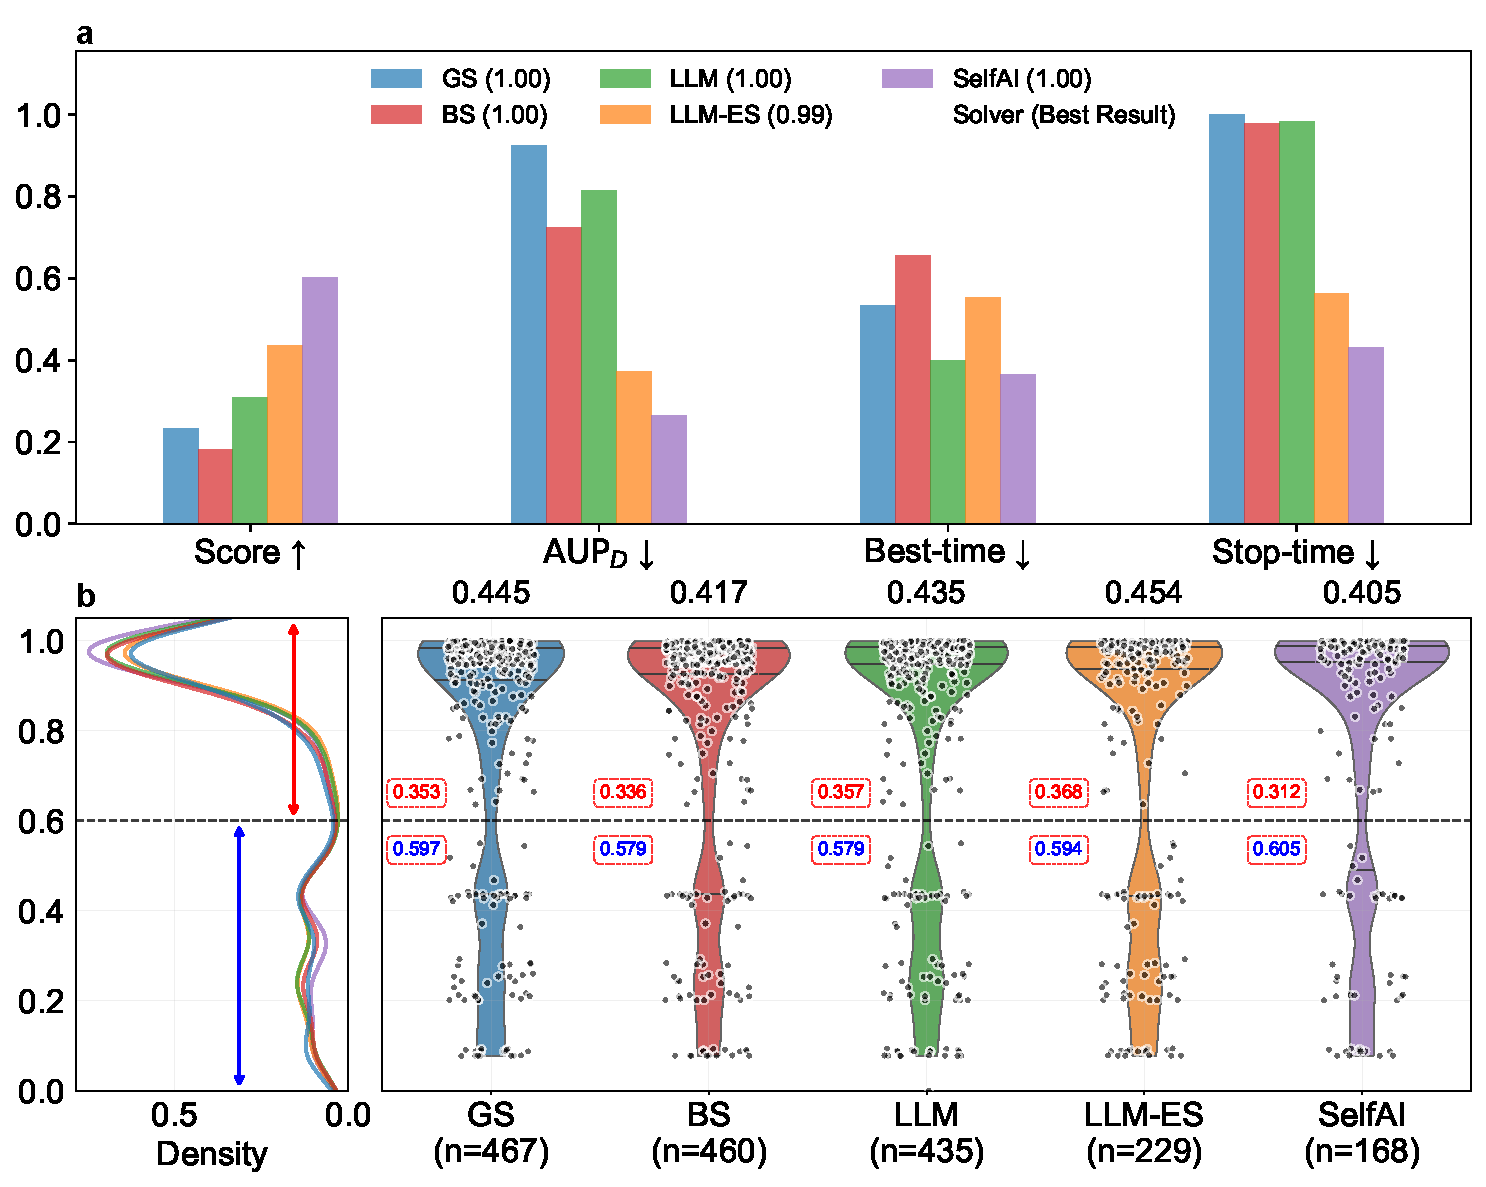
\includegraphics[width=1.0\linewidth]{figures/analysis/solver_performance_comparison2.pdf}
    \caption{\textbf{Performance comparison and efficiency-diversity trade-offs across solvers.} \textbf{a}, Normalized performance of five solvers (GS, BS, LLM, LLM-ES, and SelfAI) evaluated by Score (higher is better), $\text{AUP}_D$, Best-time, and Stop-time (lower is better). Bars indicate solver-level averages, with values in parentheses denoting the best-achieved or optimal reference performance. \textbf{b}, Outcome distributions across solvers. Left: kernel density estimates illustrating score concentration and convergence tendencies. Right: violin plots with overlaid individual trials (sample size n shown), capturing performance variability. The dashed horizontal line denotes the evaluation threshold separating low- and high-performance regimes; annotated statistics (red/blue) highlight solver behavior above and below this threshold, where broader exploration facilitates rapid escape from low-performance regions and tighter distributions in high-performance regions enable localized refinement.}
    \label{fig:comparison}
\end{figure*}

Scientific discovery across engineering~\cite{bradshaw1983studying,angelopoulos2024transforming}, physics~\cite{lupoiu2025multi,kaiser2025large}, biology~\cite{lyu2024alphafold2,nguyen2024sequence}, and medicine~\cite{yakavets2025machine,grisoni2021combining,jiang2022artificial} increasingly relies on artificial intelligence (AI) systems to support or partially automate key stages of the scientific workflow, ranging from data analysis and hypothesis generation to experimental design and execution. As scientific problems grow in scale, dimensionality, and uncertainty, computational methods have become indispensable for exploring complex hypothesis spaces. AI-assisted discovery systems hold the promise of fundamentally changing the way scientific discovery is practiced~\cite{xin2025towards}.

Most existing AI-assisted discovery systems~\cite{aira,yakavets2025machine,erps2021accelerated} adopt machine-learning-rooted paradigms, emphasizing predictive modeling on large datasets and evaluating success primarily by final performance metrics. While effective for many applications, these paradigms provide limited support for reasoning about the discovery process itself, including how hypotheses are explored, how experiments are prioritized, and how decisions are made under uncertainty. In particular, they rarely treat scientific discovery as a sequential, long-horizon decision process in which exploration strategies, resource allocation, and stopping decisions must be jointly optimized over time. Unlocking the full potential of AI in discovery, therefore, requires moving beyond performance-centric automation toward frameworks that explicitly support exploration, decision-making, and adaptation throughout the discovery trajectory.


Recent advances in large language models (LLMs)~\cite{openai2023gpt,bai2023qwen,guo2025deepseek} have significantly expanded the potential of AI systems in scientific research. Improvements in reasoning, multimodal understanding, and autonomous tool use now enable LLM-based systems to integrate planning, execution, and feedback within unified workflows. As a result, these systems can support key components of scientific discovery, including hypothesis generation, experiment design, and iterative refinement across domains~\cite{huang2022towards,ferrag2025llm}.
% 
Building on these capabilities, prior work has progressively enhanced individual aspects of the scientific workflow. Early efforts demonstrated that LLMs can extract actionable scientific knowledge to guide experiments~\cite{lin2023evolutionary,angelopoulos2024transforming} and answer domain-specific professional questions~\cite{alampara2025probing,polak2024extracting,dagdelen2024structured}. Subsequent research extended these capabilities to cross-stage planning~\cite{biomni}, automated hypothesis generation~\cite{wang2025discovery,aira,baek2025researchagent}, multimodal knowledge integration~\cite{steyaert2023multimodal,gao2025chemical}, and automated experimentation across scientific domains. These advances have led to a new generation of scientific discovery systems, ranging from AI research assistants to fully autonomous workflows capable of executing end-to-end benchmarks~\cite{king2004functional,mandal2025evaluating,ai_co_scientist}.

While these systems demonstrate the feasibility of system-level automation in scientific workflows, most existing approaches focus primarily on improving individual stages of the discovery process or optimizing final outcomes. Even recent LLM-driven optimization methods~\cite{liao2025llm4eo,jiang2025agenticsciml,kochnev2025optuna}, which infer evolutionary patterns and synthesize update rules, operate largely at the level of execution or local improvement.
% 
However, scientific discovery is inherently a sequential and strategic process that unfolds over time. It requires reasoning not only about isolated steps but also about the structure and quality of the entire exploration trajectory. Current systems rarely treat discovery as a trajectory-level decision-making problem. Consequently, they do not explicitly address fundamental challenges such as determining optimal stopping points, designing efficient exploration paths, or evaluating the structural effectiveness of discovery strategies over time.

Addressing these limitations requires a shift from execution-oriented autonomy toward cognitively oriented autonomy, in which discovery systems reason about exploration strategies, evaluate efficiency-diversity trade-offs, and adaptively decide when to stop. Motivated by this perspective, we introduce SelfAI, a self-directed, multi-agent-enabled discovery system that treats scientific discovery as a trajectory-level decision-making process. We integrate human intent, exploration reasoning, and experimental execution into a unified closed-loop framework. These are built with three modules and external tools (Fig.~\ref{fig:flowchart}a), enabling efficiency-diversity exploration in long-horizon scientific workflows. To evaluate discovery quality, we introduce two novel complementary metrics, Score (Discovery Efficiency) and $\text{AUP}_D$ (Area Under the Performance Diversity). Score aggregates across tasks, the normalized improvement over the search space together with penalties for discovering good configurations late and for stopping far from the best-found point. $\text{AUP}_D$ explicitly encodes how broadly a solver explores the search space by summarizing the performance-diversity tradeoffs across the entire trajectory, enabling detailed analysis of exploration behavior and stopping decisions in long-term searches. Together, these metrics measure quantitative assessments of exploration behavior, reasoning structure, and stopping decisions in long-term autonomous experiments.


\begin{figure*}[hbtp]
    \centering
    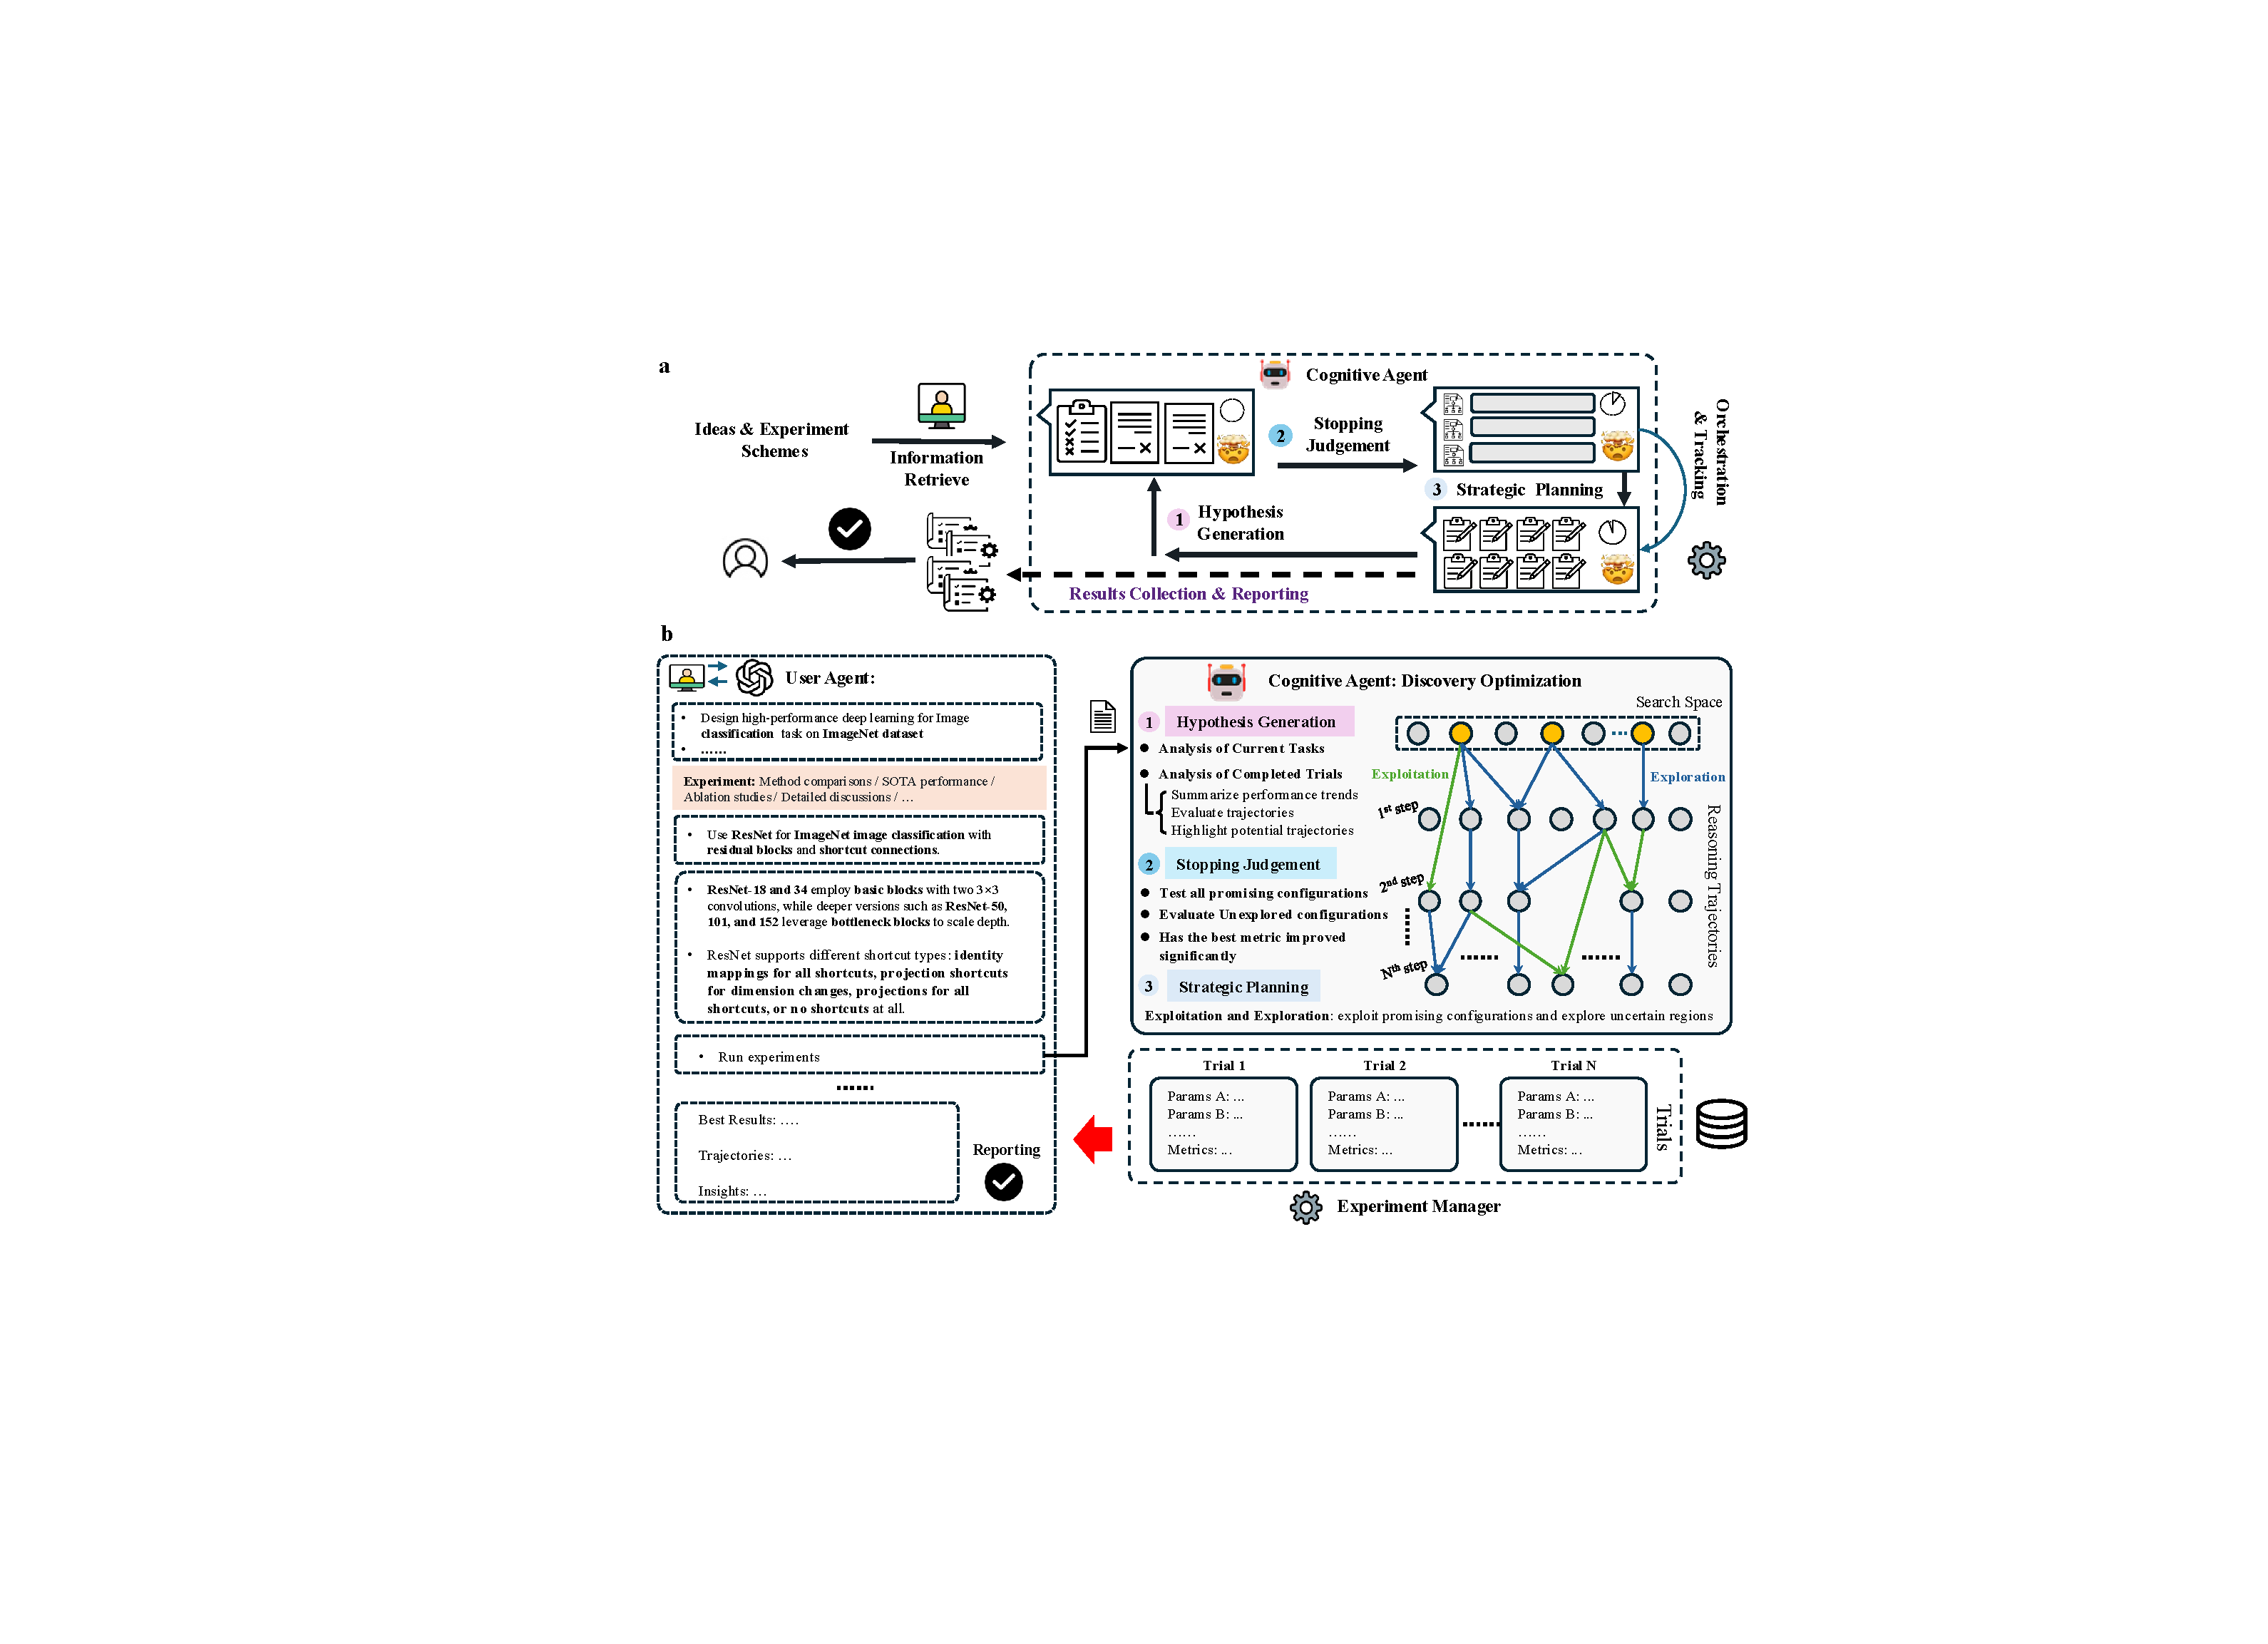
\includegraphics[width=1.0\textwidth]{figures/flowchart3-v2.pdf}
    % 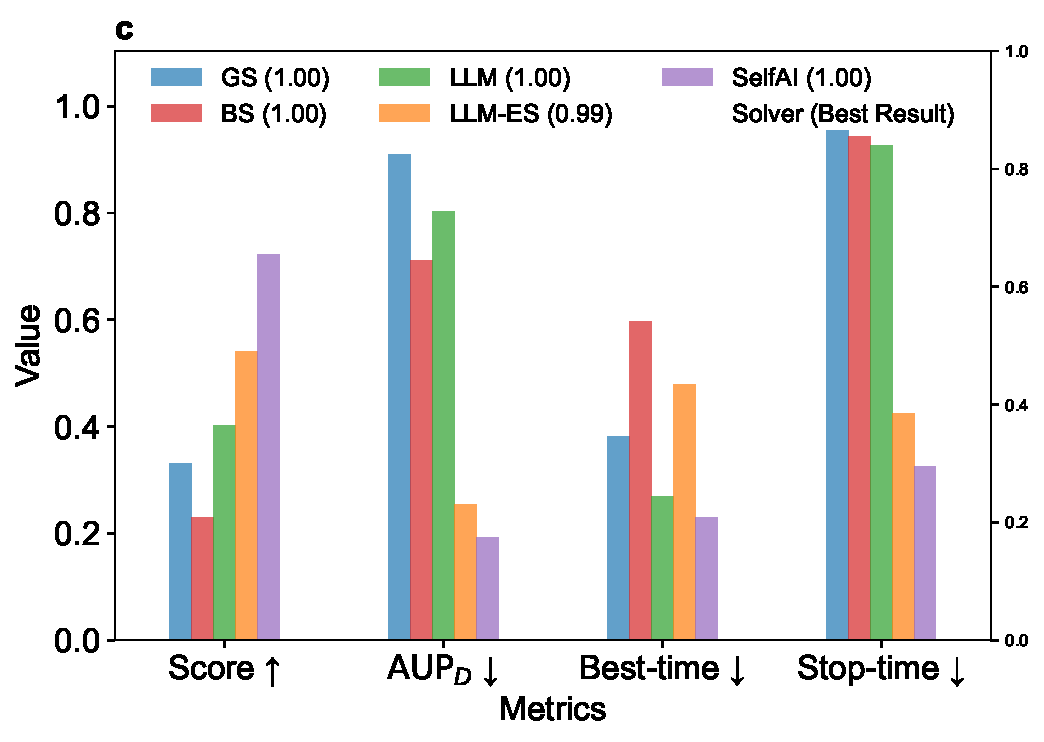
\includegraphics[width=0.49\linewidth]{figures/analysis/llm_comparison.pdf}
    % \includegraphics[width=0.49\linewidth]{figures/analysis/solver_performance_comparison.pdf}
    
    % 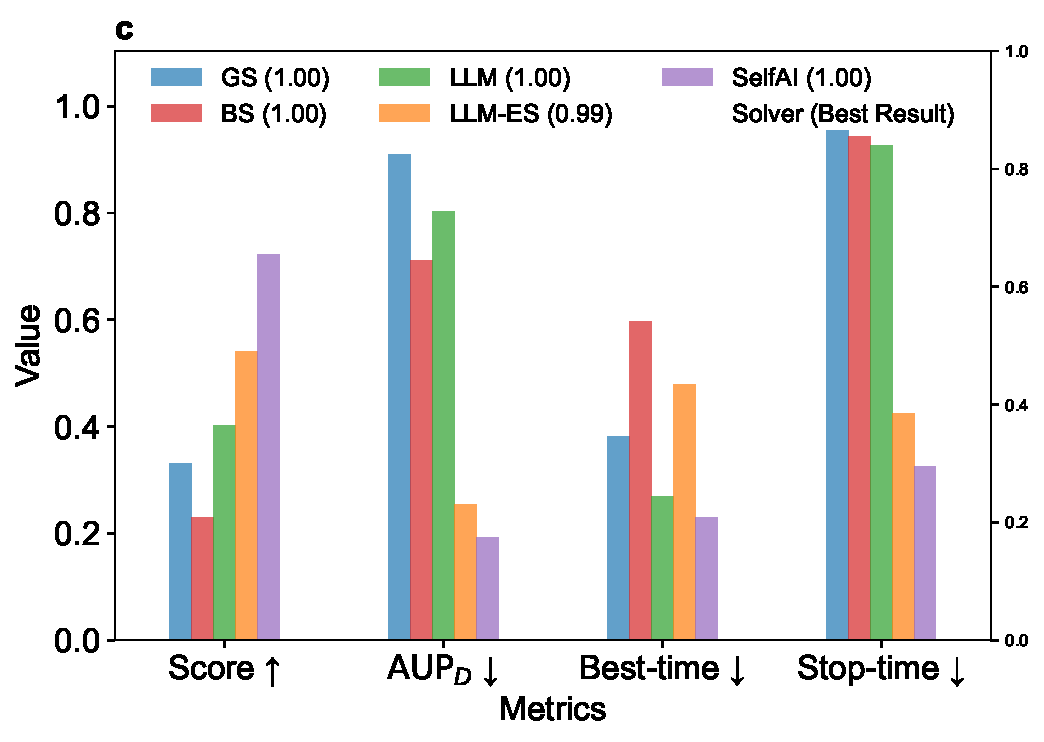
\includegraphics[width=0.7\linewidth]{figures/analysis/llm_comparison.pdf}
    % 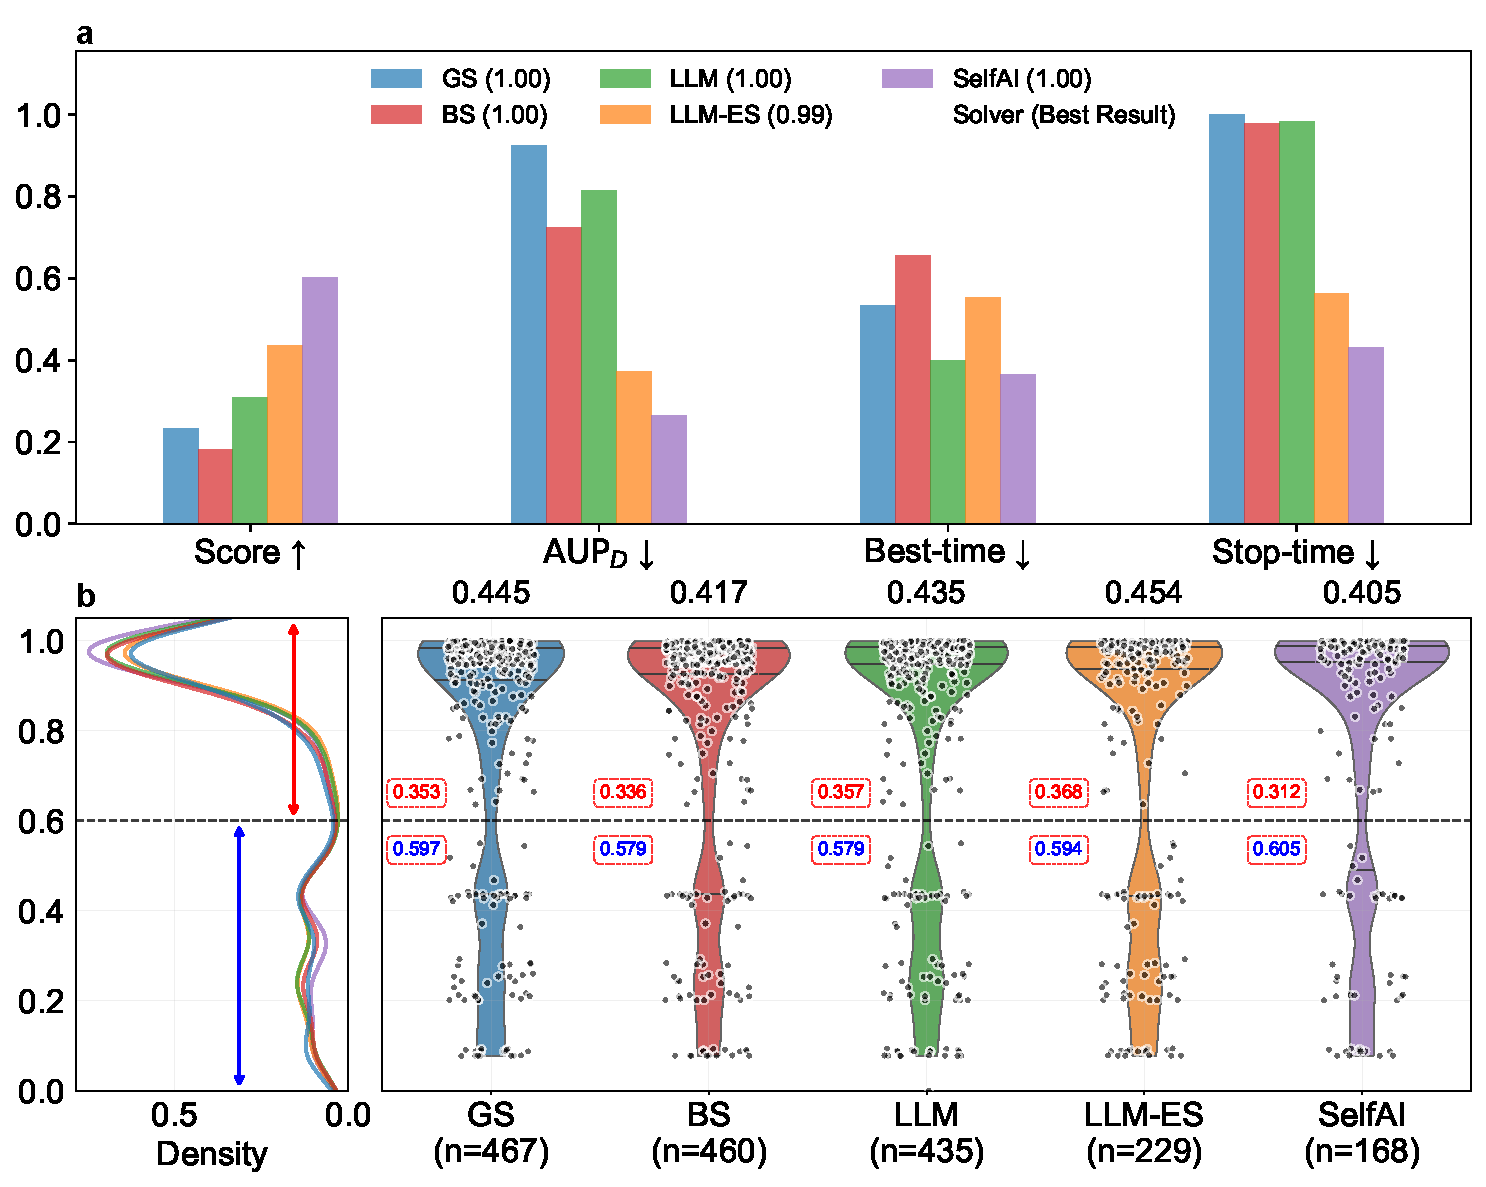
\includegraphics[width=0.7\linewidth]{figures/analysis/solver_performance_comparison2.pdf}
    \caption{\textbf{SelfAI Framework for Automated Scientific Experimentation.} \textbf{a}, Holistic architecture of the multi-agent system, which transforms various experiments in the research process into a structured workflow. \textbf{b}, User intents, comprising ideas and experiment schemes, are transformed into structured configurations via a predefined prompt. These inputs are processed through successive stages: hypothesis generation, strategic planning, trial execution, and result collection.}
    \label{fig:flowchart}
\end{figure*}
\section{Related Works}
Here, we review two lines of work closely related to long-horizon scientific discovery: agent-centric benchmarks and pipelines for scientific reasoning, and end-to-end scientific discovery systems.


{\noindent\bf Agent-Centric Benchmarks and Pipelines.} Recent agent-centric approaches focus on improving and evaluating LLM-based scientific reasoning and searching. For example, self-evolution frameworks~\citep{mlagentbench, lin2025se, aira} introduce evolution operators and flexible benchmarks to refine agent behaviors across domains. These methods have shown strong potential in improving reasoning performance but primarily rely on static or outcome-based evaluation protocols and provide limited insights into the dynamics of scientific exploration over time, such as how agents balance exploration and exploitation over long horizons. HeuriGym~\citep{chen2025heurigym} further advances this line by introducing heuristic-guided optimization during code execution and iterative refinement. It proposes metrics such as solution quality and yield quality to complement Pass@K~\cite{chen2021evaluating}, enabling a more holistic assessment of reasoning performance. However, similar to prior work, it remains centered on task-level evaluation and lacks mechanisms to model the temporal evolution of discovery processes. More recently, \cite{liu2026evox} proposes a new evolution strategy to ensure prior solutions are selected and varied to generate new candidates. Moreover, these frameworks do not provide system-level support for scalable scientific workflows, such as experiment management, hyperparameter tuning, job scheduling, and failure recovery, which are critical for real-world discovery settings. 

{\noindent\bf Scientific Discovery Systems}. 
Complementary to improving LLMs' reasoning capacities, , recent works aim to build end-to-end systems for automated scientific discovery. AI Scientist~\citep{lu2024ai, yamada2025ai, lu2026towards} introduces an agentic framework that automates key stages of the research pipeline, including hypothesis generation, experimental design, and validation, demonstrating the potential of LLMs for closed-loop scientific reasoning. Building on this paradigm, NovelSeek~\citep{novelseek} proposes a unified multi-agent system that further integrates these stages into a closed-loop pipeline, improving efficiency and coordination. Despite these advances, existing systems still face several limitations. First, they often pursue fully autonomous scientific discovery, which can lead to uncontrolled exploration and reduced reliability. In practice, scientific discovery is inherently iterative and benefits from structured human guidance; however, current systems provide limited support for effective human-in-the-loop collaboration, such as incorporating domain expertise in hypothesis refinement or steering exploration.
Second, while these systems emphasize end-to-end pipeline automation, they lack principled mechanisms for managing long-horizon exploration dynamics, including maintaining diversity, allocating computational resources, and adapting strategies over time. Third, they provide limited support for scalable and reproducible research infrastructure, particularly in large-scale experimentation and parallel training settings.

Overall, prior work either focuses on enhancing agent-centric reasoning through benchmark-driven pipelines or building end-to-end discovery systems. However, they lack a unified framework that captures the long-horizon, trajectory-level nature of scientific discovery, while simultaneously supporting process-aware evaluation and system-level scalability.  To better contextualize these gaps, Table~\ref{tab:functions_selfai} provides a systematic comparison of SelfAI and existing frameworks across three key dimensions: human-AI collaboration, long-horizon reasoning, and system-level infrastructure. As shown in the table, prior approaches either emphasize autonomous pipelines with limited controllability or focus on isolated reasoning benchmarks without supporting real-world experimentation. In contrast, SelfAI uniquely integrates human-in-the-loop interaction, trajectory-level modeling of scientific processes, and scalable experimentation capabilities. This unified design enables more controllable, adaptive, and practically deployable scientific discovery workflows.

% 

% combines LLMs with Monte Carlo Tree Search (MCTS)~\cite{swiechowski2023monte} to design domain-specific heuristics, but focuses narrowly on search strategy construction without addressing end-to-end training pipelines. RAP~\citep{RAP} leverages structured prompting to induce goal-directed behaviors, though it is constrained by static designs and lacks adaptive feedback loops.

% Overall, these limitations can be broadly categorized into three aspects: over-reliance on inherent LLM reasoning, rigid evaluation and feedback mechanisms, and persistent need for human-in-the-loop intervention.

% Overall, these limitations fall into three categories: (1) over-reliance on intrinsic LLM reasoning, (2) rigid evaluation and feedback mechanisms, and (3) continued dependence on human intervention. Compared to these approaches, our SelfAI framework (Table~\ref{tab:functions_comparison}) addresses these gaps. First, prior systems often treat LLMs as central decision-makers, increasing risks of bias, misalignment, and security vulnerabilities~\citep{zeng2024autodefense,hu2024gradient,zhang2025jbshield,wei2023jailbroken}. Second, structured critique-based refinement, while improving logical consistency, is insufficient for optimizing large-scale training, automated tuning, or robust failure recovery. Third, the need for manual specification of agent roles, reasoning processes, and optimization strategies limits scalability and efficiency~\citep{park2023generative}.



% \begin{table*}[bhtp]
% \centering
% \setlength{\tabcolsep}{4.5pt}
% \renewcommand\arraystretch{1.2}
% \caption{Comparison of SelfAI with related AI research frameworks and benchmarks across system-level, agent-specific, and task-specific capabilities.}
% \resizebox{1.0\textwidth}{!}{
% \begin{tabular}{l|cccccccc}
% \toprule
% Functions & Ours & Code LLaMA~\cite{kochnev2025optuna} & MLGym~\cite{MLgym} & AI Scientist~\cite{ai_co_scientist} & AIRA~\cite{aira} & MLAgentBench~\cite{mlagentbench} & Optuna~\cite{optuna} \\
% \midrule
% Interactive Research & \cmark & \xmark & \cmark & \xmark & \xmark & \cmark & \cmark \\ % Human-in-the-loop Collaboration
% Flexible Artifacts & \cmark & \xmark & \cmark & \cmark & \xmark & \cmark & \xmark \\
% Privacy and Security & \cmark & \xmark & \xmark & \xmark & \xmark & \xmark & \cmark \\
% \midrule
% Trajectory Analysis & \cmark & \xmark & \xmark & \xmark & \xmark & \xmark & \xmark \\
% Hypothesis Generation & \cmark & \xmark & \cmark & \cmark & \cmark & \xmark & \xmark \\
% Strategic Planning & \cmark & \xmark & \cmark & \xmark & \xmark & \xmark & \xmark \\
% Causal Inference & \cmark & \xmark & \cmark & \xmark & \xmark & \xmark & \xmark \\
% Adaptive Learning & \cmark & \cmark & \cmark & \xmark & \xmark & \xmark & \xmark \\
% \midrule
% Job Scheduling & \cmark & \xmark & \cmark & \xmark & \xmark & \xmark & \cmark \\
% Checkpoint Management & \cmark & \xmark & \xmark & \xmark & \xmark & \xmark & \xmark \\
% Experiment Tracking & \cmark & \xmark & \xmark & \xmark & \xmark & \xmark & \cmark(*) \\
% Zero-Code Parallelization & \cmark & \xmark & \xmark & \xmark & \xmark & \xmark & \xmark \\
% \midrule
% Hypothesis Optimization& \cmark & \cmark(*) & \xmark & \xmark & \xmark & \xmark & \cmark \\
% Self-Evaluation & \cmark & \xmark & \xmark & \xmark & \xmark & \xmark & \xmark \\
% Benchmark Suite & \cmark & \xmark & \xmark & \xmark & \xmark & \cmark & \xmark \\
% \bottomrule
% \end{tabular}}
% \begin{tablenotes}
% \small
% \item Note: The comparison is structured in four blocks: (1) System-level functions, (2) Cognitive functions primarily handled by the Cognitive Agent, (3) Execution functions managed by the Experiment Manager, and (4) Performance in optimization tasks. \cmark(*) denotes basic support.
% \end{tablenotes}
% \label{tab:functions_selfai}
% \end{table*}


% \begin{table*}[bhtp]
% \centering
% \setlength{\tabcolsep}{3.8pt}  % ↓ 比原来更紧凑
% \renewcommand\arraystretch{1.15}
% \caption{Comparison of SelfAI with representative AI research frameworks.}
% \resizebox{0.98\textwidth}{!}{
% \begin{tabular}{l|cccccccc}
% \toprule
% \textbf{Capabilities} & \textbf{Ours} & Code LLaMA & MLGym & AI Co-Scientist & AIRA & MLAgentBench & Optuna \\
% \midrule
% \multicolumn{9}{c}{\textit{Human--AI Collaboration}} \\
% \midrule
% Interactive Research & \cmark & \xmark & \cmark & \xmark & \xmark & \cmark & \cmark \\
% Flexible Artifacts & \cmark & \xmark & \cmark & \cmark & \xmark & \cmark & \xmark \\
% Privacy \& Security & \cmark & \xmark & \xmark & \xmark & \xmark & \xmark & \cmark \\
% \midrule
% \multicolumn{9}{c}{\textit{Long-Horizon Reasoning}} \\
% \midrule
% Trajectory Analysis & \cmark & \xmark & \xmark & \xmark & \xmark & \xmark & \xmark \\
% Hypothesis Gen./Refine & \cmark & \xmark & \cmark & \cmark & \cmark & \xmark & \xmark \\
% Strategic Planning & \cmark & \xmark & \cmark & \xmark & \xmark & \xmark & \xmark \\
% Causal Reasoning & \cmark & \xmark & \cmark & \xmark & \xmark & \xmark & \xmark \\
% Adaptive Learning & \cmark & \cmark & \cmark & \xmark & \xmark & \xmark & \xmark \\
% Self-Evaluation & \cmark & \xmark & \xmark & \xmark & \xmark & \xmark & \xmark \\
% \midrule
% \multicolumn{9}{c}{\textit{Scalable Infrastructure}} \\
% \midrule
% Job Scheduling & \cmark & \xmark & \cmark & \xmark & \xmark & \xmark & \cmark \\
% Checkpointing & \cmark & \xmark & \xmark & \xmark & \xmark & \xmark & \xmark \\
% Experiment Tracking & \cmark & \xmark & \xmark & \xmark & \xmark & \xmark & \cmark(*) \\
% Parallelization (No-Code) & \cmark & \xmark & \xmark & \xmark & \xmark & \xmark & \xmark \\
% \midrule
% \multicolumn{9}{c}{\textit{Optimization}} \\
% \midrule
% Hypothesis Optimization & \cmark & \cmark(*) & \xmark & \xmark & \xmark & \xmark & \cmark \\
% Benchmark Suite & \cmark & \xmark & \xmark & \xmark & \xmark & \cmark & \xmark \\
% \bottomrule
% \end{tabular}}
% \begin{tablenotes}
% \small
% \item \textbf{Note:} \cmark(*) denotes partial support.
% \end{tablenotes}
% \label{tab:functions_selfai}
% \end{table*}



\begin{table*}[bhtp]
\centering
\setlength{\tabcolsep}{4.5pt}
\renewcommand\arraystretch{1.2}
\caption{Comparison of SelfAI with related AI research frameworks and benchmarks across system-level, agent-specific, and task-specific capabilities.}
\resizebox{0.98\textwidth}{!}{
\begin{tabular}{l|cccccccc}
\toprule
\textbf{Capabilities} & \textbf{Ours} & Code LLaMA & MLGym & AI Scientist & AIRA & MLAgentBench & Optuna \\
\midrule
\multicolumn{8}{c}{\textit{Human-AI Collaboration}} \\
\midrule
Interactive Research & \cmark & \xmark & \cmark & \xmark & \xmark & \cmark & \cmark \\
Flexible Artifacts & \cmark & \xmark & \cmark & \cmark & \xmark & \cmark & \xmark \\
Privacy \& Security & \cmark & \xmark & \xmark & \xmark & \xmark & \xmark & \cmark \\
\midrule
\multicolumn{8}{c}{\textit{Long-Horizon Reasoning}} \\
\midrule
Trajectory Analysis & \cmark & \xmark & \xmark & \xmark & \xmark & \xmark & \xmark \\
Hypothesis Generation & \cmark & \xmark & \cmark & \cmark & \cmark & \xmark & \xmark \\
Strategic Planning & \cmark & \xmark & \cmark & \xmark & \xmark & \xmark & \xmark \\
Causal Reasoning & \cmark & \xmark & \cmark & \xmark & \xmark & \xmark & \xmark \\
In-context Learning & \cmark & \cmark & \cmark & \xmark & \xmark & \xmark & \xmark \\
Self-Evaluation & \cmark & \xmark & \xmark & \xmark & \xmark & \xmark & \xmark \\
\midrule
\multicolumn{8}{c}{\textit{Scalable Infrastructure}} \\
\midrule
Job Scheduling & \cmark & \xmark & \cmark & \xmark & \xmark & \xmark & \cmark \\
Checkpointing & \cmark & \xmark & \xmark & \xmark & \xmark & \xmark & \xmark \\
Experiment Tracking & \cmark & \xmark & \xmark & \xmark & \xmark & \xmark & \cmark(*) \\
Parallelization (No-Code) & \cmark & \xmark & \xmark & \xmark & \xmark & \xmark & \xmark \\
\midrule
\multicolumn{8}{c}{\textit{Optimization}} \\
\midrule
Hypothesis Optimization & \cmark & \cmark(*) & \xmark & \cmark & \xmark & \xmark & \cmark \\
Benchmark Suite & \cmark & \xmark & \xmark & \xmark & \xmark & \cmark & \xmark \\
\bottomrule
\end{tabular}}
\begin{tablenotes}
\small
\item \textbf{Note:} \cmark(*) denotes partial or basic support. Compared to prior work, SelfAI uniquely integrates human-in-the-loop collaboration, long-horizon trajectory modeling, and scalable infrastructure within a unified framework.
\end{tablenotes}
\label{tab:functions_selfai}
\end{table*}

\section{Methods}
% I will update the following content with NeurIPS style. 
% use mathematical description to convert agentic process

\subsection{SelfAI system}
\label{sec:method}
The SelfAI system operates in an integrated loop, comprising three core agents: User Agent, Cognitive Agent, and Experiment manager, which together constitute the overall experimental pipeline in Fig.~\ref{fig:flowchart}. It consists of three components: a User Agent for intent formalization, a Cognitive Agent for iterative decision-making, and an Experiment Manager for experiment orchestration and management. Before illustrating the details of SelfAI, we first situate SelfAI within the landscape of existing AI-assisted research frameworks by examining their functional coverage (Table~\ref{tab:functions_selfai}).

\paragraph{User Agent}
As illustrated in Fig.~\ref{fig:flowchart}b, User Agent serves as the user interface through which high-level research intent is translated into structured, machine-readable experimental specifications. Its primary function is to formalize natural-language objectives provided by users into a standardized configuration that defines the experimental task for the SelfAI system. For example, user requests such as “Design high-performance deep learning for image classification task on the ImageNet dataset” or “Identify the most influential method for image classification” are reformulated into precise experimental specifications. Specifically, User Agent maps user-provided descriptions of research goals, constraints, and preferences into a task-specific YAML configuration. This configuration explicitly specifies basic ideas, optimization objectives, the experimental search space, trial budget, and historical trial data (as shown in Supplementary Sect.~\ref{sec:supp_user_agent}). The resulting YAML file serves as the sole interface between user intent and downstream system components, including Cognitive Agent and Experiment Manager. Consequently, User Agent encodes the user’s research intent into a fixed configuration schema, which is implemented via a predefined prompt template. All interactions are restricted to the generation and refinement of the structured configuration, and users do not directly manipulate experimental parameters or outcomes once the configuration is finalized. 


\paragraph{Cognitive agent}
\label{sec:cognitive}
Cognitive Agent performs iterative decision-making within the SelfAI framework by operating on structured experimental inputs and conducting trajectory-level analysis across multiple iterations. To support long-horizon optimization, Cognitive Agent operates in three functional stages: hypothesis generation, strategic planning, and stopping judgment. Hypothesis generation identifies promising regions of the search space based on accumulated experimental outcomes. Strategic planning translates these hypotheses into concrete experimental proposals that balance refinement of high-performing configurations with exploration of under-sampled or uncertain regions. Stopping judgment evaluates accumulated experimental evidence to determine whether continued experimentation is warranted under the current exploration strategy. At each iteration, Cognitive Agent receives a task-specific experimental configuration from User Agent, along with accumulated experimental histories and performance metrics from Experiment Manager. These inputs are provided in a structured format and define the current state of the search process. Using the accumulated evidence, Cognitive Agent evaluates experimental trajectories, assesses observed performance trends, and estimates coverage of the explored search space. Based on this analysis, it generates candidate experimental configurations for subsequent exploration. In addition to proposing new experiments, the Cognitive Agent produces a stopping decision based on trajectory-level evaluation of completed trials, including comparison with the initial configuration, assessment of diminishing returns in recent performance improvements, and estimation of the potential value of remaining unexplored regions. The outputs of Cognitive Agent consist of candidate experimental configurations for the next iteration and a stopping signal indicating whether the current exploration process should be terminated. Detailed implementation, including the prompt templates used for hypothesis generation, strategic planning, and stopping judgment, is provided in the Supplementary Materials~\ref{sec:supp_cognitive}.


\paragraph{Experiment manager}
\label{sec:exp_management}
Experiment Manager is responsible for experiment orchestration and recovery, including resource management, task allocation, and progress tracking (Fig.~\ref{fig:flowchart}b). These capabilities enable efficient coordination of multi-instance parallel optimization, maximize resource utilization, and enhance training robustness.

1) {\bf Resource Management}. Experiment Manager monitors resource consumption and dynamically allocates available GPU, TPU, and memory resources. This granular allocation optimizes workload distribution across computing units and ensures stable execution of all trials.

2) {\bf Fault recovery and Checkpoint Reconnection}. In case of system interruptions or suboptimal model performance, Experiment Manager reports failures to Cognitive agent. Experiment Manager performs preliminary diagnostics, identifies potential issues, adjusts training parameters, and resumes training from the latest checkpoint.

3) {\bf Multi-Instance Parallel Optimization}. SelfAI instantiates each user program to run across diverse physical environments, independent of the target program framework. Experiment Manager coordinates multi-instance parallel training, synchronizes execution, and concurrently tests various configurations, thereby shortening overall training time and improving generalization across datasets and model parameters. For each parallel experiment, Experiment Manager identifies and supplies the necessary runtime parameters, ensuring experiments are conducted under the same environment optimized by Cognitive agent.


\subsection{
Evaluation for reasoning trajectories}
\label{sec:evaluation_reasoning}
While the reasoning process of LLMs in problem-solving often generates a diverse range of discrete insights and multiple potential chains of thought, this diversity, though valuable for exploration and exploitation, can pose a challenge to coherent reasoning evaluation across various experimentation and discovery phases. We propose a systematic evaluation metric that captures both the diversity of reasoning perspectives and the overall coherence of the reasoning process, ensuring a more robust and comprehensive assessment of reasoning capabilities.


\noindent\textbf{.}
We formalize a reasoning trajectory for task i as a finite sequence of evaluations
\begin{equation}
    \mathcal{T} = \{v_{i,t}\}
\end{equation}

\noindent\textbf{Optimal Stopping Criteria.}
In this work, we collected the best value point and the stop point from trials. Based on Optimal Stopping Criteria~\cite{hill2009knowing}, we can define the following measure formulas,
\begin{align}
    % & \text{SUCC} = \frac{1}{N} \sum^{N-1}_{i=0} S_{i} \\
    & \text{Gain} = \frac{1}{N} \sum^{N-1}_{i=0} \frac{v^*_{i,t} - v_{i,\min}}{v_{i,\max} - v_{i, \min}}
     \\
    & t_{\text{best}} = \frac{1}{N} \sum^{N-1}_{i=0}t^{\text{best}}_i = \frac{1}{N} \sum^{N-1}_{i=0} \frac{m_i}{M_i} \\
    & t_{\text{stop}} = \frac{1}{N} \sum^{N-1}_{i=0}t^{\text{stop}}_i = \frac{1}{N} \sum^{N-1}_{i=0} \frac{n_i}{M_i}
\end{align}
and
% \begin{equation}
%     S_{i} =
%     \begin{cases}
%         1, & \text{if } v_i^* == v_{\max} \\
%         0, & \text{otherwise}
%     \end{cases}
% \end{equation}
% $\text{SUCC}$ denotes that the obtained result is the best value. Then, f
where $N$ is the number of tasks. For the $i$-th task, $M_i$ is the number of completed trials. $m_i$ is the best value point index. $t_i^{\text{best}}$ is the cost of the best value. In addition, we set the stop point index, $n_i$, and $t_i^{\text{stop}}$ is better when $n_i$ is closer to the best value point index. $S_i$ means the binarized value.

To obtain a comprehensive measure, we combine the last three measures, i.e., $\text{Rel}$, $t_{\text{best}}$, and $t_{\text{stop}}$, where we utilize  $\text{Rel}$ in underestimated penalty, then $t_{\text{best}}$ and $t_{\text{stop}}$ are the time penalty ($P_\text{best}$ and $P_\text{stop}$). Thus, the total penalty is
\begin{align}
    % P_{\text{best}} &= w_{\text{best}} \cdot t^{\text{best}}_i \notag\\
    % P_{\text{stop}} &= w_{\text{stop}} \cdot t^{\text{stop}}_i \\
    P_{\text{total}} &= \frac{t_i^{\text{stop}} + t_i^{\text{best}}}{2}
\end{align}

Finally, the score is denoted as
\begin{align}
    & \text{Score} = \frac{1}{N}\sum^{N-1}_{i=0} \text{Gain} \cdot (1-P_{total})
\end{align}
\noindent \textbf{Best Approximation/Candidate} In \cite{MLgym}, performance profiles and the AUP aim to measure available rates across $\texttt{m}$ tasks, where all performance metrics are threshold $\tau$, performance profiles ($ \rho_\texttt{m}(\tau)$) are computed as thresholds in all metrics (sorted by ascending) in the current task.
\begin{equation}
    \text{AUP}_\texttt{m} = \int^{\tau_{\max}}_1 \rho_\texttt{m}(\tau) d\tau
\end{equation}
It is noted that the above performance profile and $\text{AUP}_\texttt{m}$ score cannot measure the diversity of reasoning. Therefore, we rewrite the performance profile and AUP score:

First, the performance profile is defined in all completed trials $M_i$ in $i$-th task and the overall search space $\mathcal{H}$, as follows 
\begin{equation}
    r_i =
    \begin{cases}
         \frac{\max{\{v_k:\, k \in \mathcal{H}\}}}{v_i},\, \text{ascend}  
         \\
         \\
         \frac{v_i}{\min{\{v_k:\, k \in \mathcal{H}\}}},\, \text{descend}
    \end{cases}
\end{equation}
where ascend/descend denotes that the value is larger/smaller and the performance is better. For all trials, $\tau$ is the set of all obtained $r_i$ values. Then, we consider all completed trials $M_i$ in $i$-th task, 
\begin{align}
    & \rho_i(\tau) = \begin{cases}
         |\{k \in M_i: r_k >= \tau \}|, &\text{ascend} \\
        |\{k \in M_i: r_k <= \tau \}|, & \text{descend}
    \end{cases}
\end{align}
which captures how many evaluated configurations exceed a given performance threshold $\tau$. $\rho_i(\tau)$ is the cumulative distribution curve of the trajectory. 

The area term aggregates the overall concentration of strong configurations along the performance axis:
\begin{equation}
    A = \frac{1}{N} \sum^{N-1}_{i=0} \int_{\tau_{\min}}^{\tau_{\max}} \rho_{i}(\tau)d\tau.
\end{equation}
To capture the temporal asymmetry of discovery, we compute the centroid
\begin{equation}
    G = \frac{1}{A} \int_{\tau_{\min}}^{\tau_{\max}} x \cdot \rho_i(\tau) \, d\tau,
\end{equation}
and define the skewness
\begin{equation}
    S = \int_{\tau_{\min}}^{\tau_{\max}} \left( \frac{x}{G} \right)^3 \rho(x) \, d\tau.
\end{equation}
Since $S$ may be unbounded and may take both positive (left-skewed) and negative (right-skewed) values, we normalize it via a reference skewness value $S_\text{base}$ from the GS method and a smooth monotonic mapping:
\begin{align}
    & S’ = 1-\frac{S-S_\text{base}}{S_\text{base}}, \\
    & S' = \frac{\tanh(S) + 1}{2}, S' \in (0, 1).
\end{align}
Finally, the Area Under the Performance-Diversity curve ($\text{AUP}_D$) is defined as
\begin{equation}
    \text{AUP}_D = A / S',
\end{equation}
where trajectories that exhibit earlier concentration of high-performing configurations obtain larger and thus smaller $\text{AUP}_D$ values, whereas trajectories that concentrate improvements later yield smaller and therefore larger values.
\section{Experiment}

The benchmark comprises 12 tasks spanning six scientific categories, including scientific computing, machine learning, computer vision, medical image analysis, and drug discovery (Table~\ref{tab:task_list}). All benchmark data are collected from real experimental runs, with several tasks corresponding to configurations reported in published literature. The tasks cover both discrete and continuous search spaces and range from low- to high-dimensional settings. To simulate realistic user-system interaction, each task provides background information to the LLM to support intent interpretation. Most datasets are generated through systematic grid-based exploration, while LCBench and the Chagas EP20 drug discovery dataset are constructed from Bayesian optimization trajectories. LCBench is a widely used AutoML benchmark~\cite{zimmer2021auto}. All tasks are organized as YAML specifications containing metadata, task definitions, concise problem descriptions, search spaces, and trial records.
\subsection{Compared methods and evaluation setup}
We evaluate SelfAI across all 12 benchmark tasks and compare it with classical optimization methods, including grid search and the Tree Parzen Estimator (TPE) optimizer~\cite{optuna}, referred to as BS. To assess robustness across model families, we instantiate SelfAI with different language-model backbones, including OpenAI-o3~\cite{openai2023gpt}, Llama3.3~\cite{llama}, Qwen2.5~\cite{bai2023qwen}, and DeepSeek-R1~\cite{guo2025deepseek}. All methods are evaluated under identical computational settings. Reasoning traces are retained for analysis and reproducibility. For all trials, the random seed is fixed, and the temperature is set to zero. The detailed settings of the benchmark are available in the Supplementary Materials.

\begin{table}[h!]
\centering
\setlength{\tabcolsep}{4pt}
\renewcommand{\arraystretch}{1.2}
\caption{List of tasks in SelfAI with different hyperparameters for multiple tasks and datasets.}
\begin{tabular}{@{}lllcccc@{}}
\toprule
\textbf{Category} & \textbf{Method} & \textbf{Task} & \textbf{Dim} & \textbf{Count} & \textbf{Ref.} \\ 
\midrule
\multirow{1}{*}{Scientific Computing} & Tensor Network & Image Completion & 3 & 64 & \cite{tw} \\  
\hline
\multirow{3}{*}{Machine Learning} 
 & Random Forest & Pricing Prediction & 5 & 162 & \cite{boston} \\
 & LSTM & Sentiment Analysis & 2 & 20 & \cite{sentiment_analysis} \\ 
 & GraphSAGE & Node Classification & 22 & 25 & \cite{yan2023unreal} \\ 
 \hline
\multirow{5}{*}{Computer Vision} & SIREN & Image Denoising & 2 & 25 & \cite{sitzmann2020implicit} \\
 & SIREN & Image Segmentation & 2 & 25 & \cite{sitzmann2020implicit} \\
 & ResNet & Image Classification & 4 & 9 & \cite{resnet} \\ 
 & MAE & Image Classification & 2 & 20 & \cite{mae} \\ 
 & FashionMnist-NN & Image Classification & 5 & 2000 & \cite{zimmer2021auto} \\ 
\hline
\multirow{2}{*}{Medical Image Analysis} & nnUnet & BraTS~\cite{brats} & 3 & 18 & \cite{nnunet} \\
 & nnUnet-revisited & BTCV~\cite{btcv} & 5 & 19 & \cite{nnunet_revisit} \\
Drug Discovery & DNN & Bioactivity Prediction & 4 & 30 & \cite{korotcov2017comparison} \\
\bottomrule
\end{tabular}
\label{tab:task_list}
\end{table}


\begin{table}[h]
    \renewcommand\arraystretch{1.2}
    \setlength{\tabcolsep}{2pt}
    \centering
    \caption{Averaged performance comparison of SelfAI across different tasks.}
    \label{tab:hit}
    % \resizebox{\textwidth}{!}{
    \begin{tabular}{llccccccc}
    \toprule
    Solver & Score$\uparrow$ & $\text{AUP}_D\downarrow$ & Best-Time$\downarrow$ & Stop-Time$\downarrow$ & Best Result$\uparrow$ & Hit-Rate$\uparrow$ & Rank \\
    \midrule
    GS & 0.2453 & 1.0000 & 0.5094 & 1.0000 & 1.0000 & 1.0000 & 14 \\
    BS & 0.1927 & 0.8106 & 0.6265 & 0.9881 & 1.0000 & 1.0000 & 15 \\
     LLM & 0.3526 & 0.7638 & 0.2949 & 1.0000 & 1.0000 & 0.9286 & 13 \\
    LLM-ES & 0.5294 & 0.2349 & 0.4691 & 0.4582 & 0.9981 & 0.6429 & 3 \\
    \midrule
    % The following results are from selfai using different LLMs.
    Qwen2.5-7b      & 0.5562 & 0.2154 & 0.4805 & 0.3945 & 0.9957 & 0.7857 & 2 \\
    Qwen2.5-14b     & 0.5015 & 0.3310 & 0.4926 & 0.4997 & 0.9969 & 0.7857 & 5 \\
    Qwen2.5-32b     & 0.4287 & 0.4684 & 0.5252 & 0.6133 & 0.9972 & 0.7857 & 10 \\
    Qwen2.5-72b     & 0.4189 & 0.5358 & 0.4531 & 0.7087 & 0.9995 & 0.8571 & 11 \\
    DeepSeek-r1-7b  & 0.4769 & 0.1802 & 0.7020 & 0.3093 & 0.9927 & 0.5000 & 8 \\
    DeepSeek-r1-14b & 0.4793 & 0.3956 & 0.4953 & 0.5100 & 0.9948 & 0.7143 & 7 \\
    DeepSeek-r1-32b & 0.4989 & 0.3476 & 0.4535 & 0.5433 & 0.9933 & 0.7857 & 6 \\
    DeepSeek-r1-70b & 0.4556 & 0.3513 & 0.5392 & 0.5299 & 0.9962 & 0.7143 & 9 \\
    Llama3.3-70b    & 0.3625 & 0.5483 & 0.5099 & 0.7271 & 0.9683 & 0.7143 & 12 \\
    GPT4-o3-mini    & 0.6433 & 0.2259 & 0.3168 & 0.3961 & 0.9989 & 0.8571 & 1 \\
    GPT4-o3         & 0.5140 & 0.2284 & 0.5477 & 0.3961 & 0.9966 & 0.6429 & 4 \\
    \bottomrule
    \end{tabular}
    % }
\end{table}


\section{Evaluation}

To characterize efficiency-diversity trade-offs in long-horizon exploration, we propose four metrics: Score, $\text{AUP}_D$, $t_{\text{best}}$, and $t_{\text{stop}}$ (Fig.~\ref{fig:comparison}a), the details of which are described in Sect.~\ref{sec:evaluation_reasoning}. These metrics not only reflect final performance but also explicitly capture when high-quality solutions are discovered, how broadly the search space is explored, and how efficiently exploration is terminated. Score aggregates normalized improvement while penalizing both delayed discovery of optimal configurations and prolonged exploration after performance plateaus. $\text{AUP}_D$ (Area Under the Performance-Diversity Curve) quantifies the diversity of explored high-quality solutions and summarizes how performance gains are distributed along the discovery trajectory. The metrics $t_{\text{best}}$ and $t_{\text{stop}}$ denote the normalized time first to identify the best result and the time at which exploration terminates, respectively. An effective solver minimizes both quantities, achieving early discovery while avoiding unnecessary trials. In this framework, effective exploration strategies attain a high Score with a relatively low $\text{AUP}_D$, indicating efficient discovery with minimal wasted exploration. Detailed per-task comparisons of Score, $\text{AUP}_D$, $t_{\text{best}}$, and $t_{\text{stop}}$ are provided in the Supplementary Materials~\ref{sec:supp_details_benchmark}.



Across 12 heterogeneous tasks and language-model backbones (Supplementary Sect. ~\ref{sec:supp_details_benchmark}), these results demonstrate that SelfAI yields consistent trajectory-level benefits. SelfAI does not merely improve convergence accuracy but fundamentally reorganizes exploration dynamics in long-horizon scientific discovery.  By reallocating experimental effort away from diminishing-return regions toward structurally informative areas of the search space, SelfAI implements a policy-adaptive exploration strategy that aligns with identifiable principles of long-horizon scientific discovery.

\subsection{Emergent principles of long-horizon scientific discovery}
We further investigate whether long-horizon scientific discovery exhibits consistent, task-agnostic principles when guided by trajectory-aware reasoning. Fig.~\ref{fig:siren_surface} illustrates these trajectory-level dynamics in the hyperparameter search landscape for image segmentation using SIREN (Sect.~\ref{sec:case_studies}). From principles of long-horizon scientific discovery, trajectory-level dynamics follow a characteristic three-stage trajectory: rapid escape from low-efficiency regions, early concentration of effort in high-potential areas, and termination near the optimal configuration. This structured progression highlights the central role of strategic trial allocation and adaptive stopping in the efficiency of long-horizon exploration. 

Aggregated performance across tasks and domains reveals additional trajectory-level regularities (Fig.~\ref{fig:bar_score_aup}). Despite task-dependent variations in relative rankings (Supplementary Fig.~\ref{fig:rank_heatmap}), SelfAI consistently achieves high Scores while maintaining relatively low $\text{AUP}_D$ values across heterogeneous tasks and language-model backbones. These results indicate that efficient discovery trajectories can be organized according to shared principles that are not tied to any single task or domain. 

Model scale alone does not systematically improve long-horizon discovery behavior. Larger models often sustain prolonged exploration of alternative hypotheses, leading to delayed commitment and reduced adaptability under fixed experimental budgets. In contrast, small and mid-sized models often exhibit more stable cumulative progress, earlier concentration on informative regions, and more reliable stopping behavior. These observations show that baseline LLM solvers relying on exhaustive exploration without principled stopping often exhaust their search budgets (Fig.~\ref{fig:flowchart}). In contrast, SelfAI-enabled solvers achieve substantially higher hit rates while terminating exploration significantly earlier. Notably, final performance is often near saturation across methods, with the best results differing only marginally. Nevertheless, significant differences exist in performance and diversity metrics, revealing substantial differences in identifying high-quality configurations and effectiveness in avoiding redundant experiments.



\begin{figure*}[t]
    \centering
    \begin{tabular}{c}
        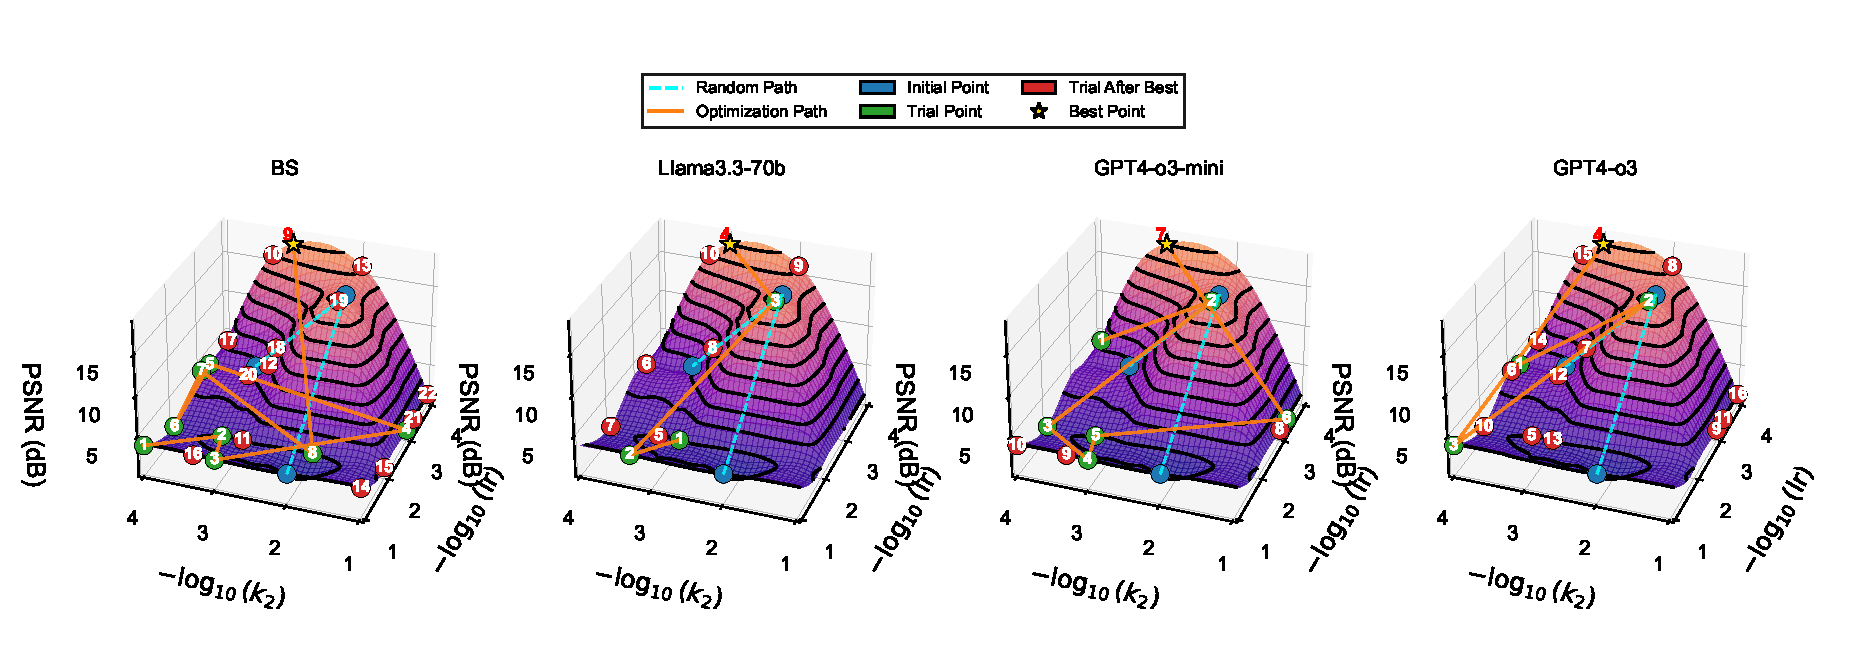
\includegraphics[width=1.0\textwidth]{figures/siren/cols/multi_model_comparison1.pdf} \\
        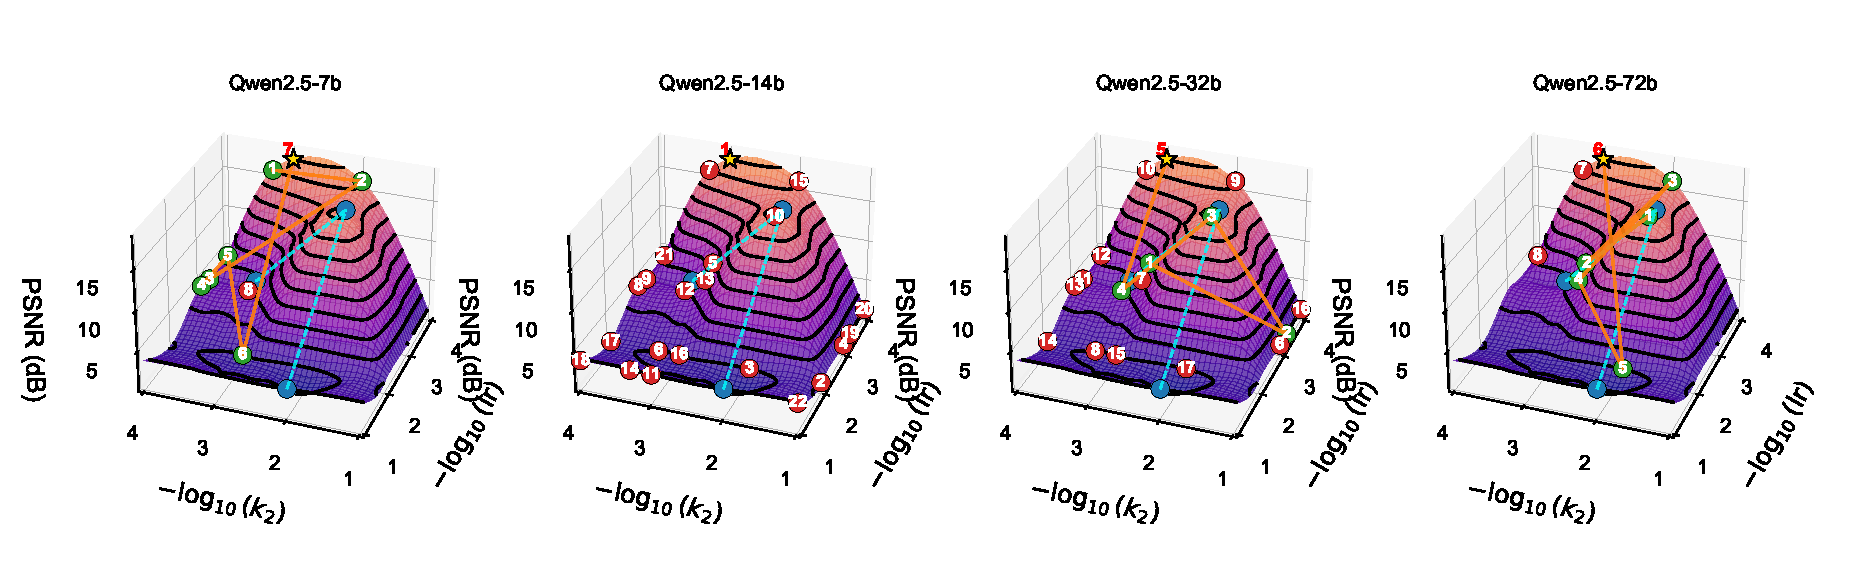
\includegraphics[width=1.0\textwidth]{figures/siren/cols/multi_model_comparison2.pdf} \\
        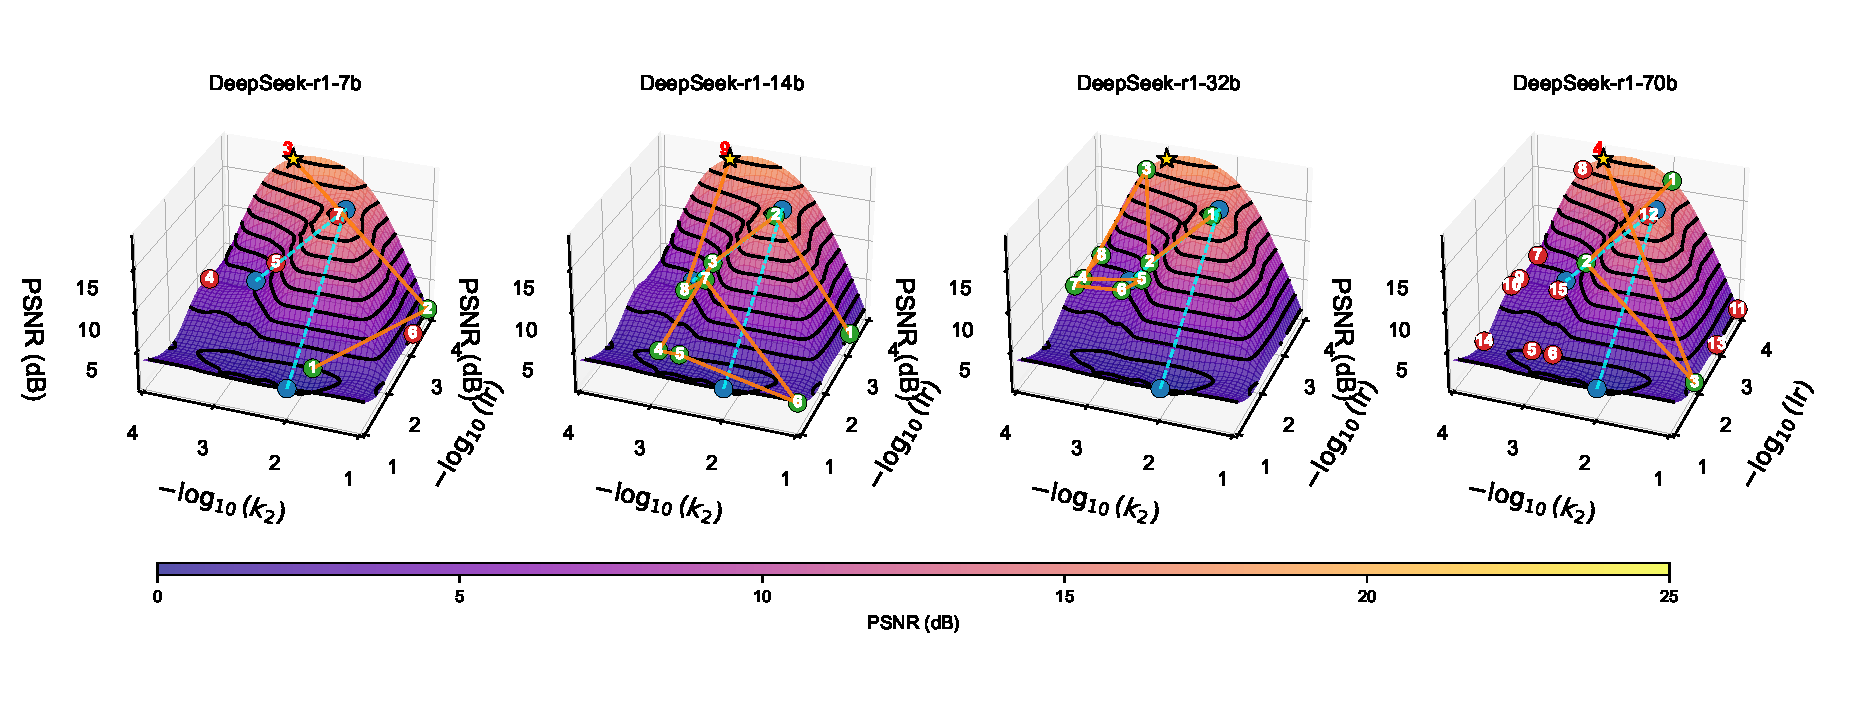
\includegraphics[width=1.0\textwidth]{figures/siren/cols/multi_model_comparison3.pdf} \\
    \end{tabular}
    \caption{Illustration of the optimized trajectory for the SIREN method for image segmentation. Green points are suggested points before reaching the optimal points. Red points are redundant suggestions when reaching out to the optimal points and failing to stop trials. The $\star$ is the optimal point. We show the serialization recommendations provided by LLM through the labeled numbers.}
    \label{fig:siren_surface}
\end{figure*}

\section{Conclusion}
In this paper, we present SelfAI, a unified framework for long-horizon scientific discovery that integrates human--AI collaboration, trajectory-level reasoning, and scalable experimentation infrastructure. Unlike prior approaches that either emphasize fully autonomous pipelines or focus on isolated reasoning benchmarks, SelfAI supports interactive and controllable discovery processes, reflecting the inherently iterative and expert-driven nature of scientific research.
In addition to system design, SelfAI introduces a process-aware evaluation perspective that moves beyond outcome-based metrics toward trajectory-level analysis. This enables a more comprehensive assessment of scientific discovery by capturing not only final results but also intermediate exploration behaviors, including diversity, efficiency, and adaptation over time. By jointly unifying collaboration, reasoning, evaluation, and infrastructure, SelfAI bridges the gap between controlled benchmarking environments and real-world scientific workflows, providing a practical and extensible foundation for reliable and adaptive scientific discovery.




%%%%%%%%%%%%%%%%%%%%%%%%%%%%%%%%%%%%%%%%%%%%%%%%%%%%%%%%%%%%
\bibliographystyle{plain}
\bibliography{reference}


\appendix
\input{5-appendix}


%%%%%%%%%%%%%%%%%%%%%%%%%%%%%%%%%%%%%%%%%%%%%%%%%%%%%%%%%%%%

\newpage
\input{checklist.tex}


\end{document}